\documentclass{article}

\usepackage[margin=1in]{geometry}
\usepackage{graphicx}
\usepackage{caption}
\usepackage{hyperref}

\setlength{\emergencystretch}{3em}
\setcounter{secnumdepth}{0}
\renewcommand{\thefigure}{S\arabic{figure}}
\captionsetup[figure]{name=Fig.}

\title{Supplementary Materials}
\author{}
\date{}

\begin{document}

\maketitle

\section*{Supplementary Materials}

\subsection*{S1. Dataset construction and annotation}

Field images were collected from two vineyard sites in Guangxi, China
between April and August 2024. Images were captured using two consumer
smartphones at a distance of approximately 15--20 cm. Each image focused
on a single leaf. Images with severe blur, strong direct sunlight,
incomplete leaves, or heavy occlusion were excluded before annotation.

Leaf and lesion regions were annotated using LabelMe. Two binary masks
were generated for each image: a leaf mask for leaf/background
segmentation and a lesion mask for lesion/non-lesion segmentation. Three
datasets were then constructed: the original full-field images for leaf
segmentation, cropped leaf regions for lesion segmentation, and original
images paired with lesion masks for single-stage comparison.

\subsection*{S2. Additional model design details}

The first stage uses DeepLabV3+ because its multi-scale context
aggregation is suitable for complete leaf extraction under complex
backgrounds. MobileNetV3 was selected as a compact backbone, and its SE
attention was replaced by SimAM to improve spatial sensitivity without
adding learnable parameters.

The second stage uses a U-Net framework because skip connections and
decoder reconstruction are effective for small lesion regions.
EfficientNet-B0 replaces the heavier VGG16 encoder to reduce parameter
cost while retaining multi-scale feature extraction. RepConv is used in
the decoder because it provides multi-branch representation during
training and can be re-parameterized into a single convolution during
inference.

\subsection*{S3. Additional ablation settings}

For leaf segmentation, the compared segmentation architectures included
U-Net, DeepLabV3+, PSPNet, HRNet, and SegFormer. Backbone comparison was
conducted within DeepLabV3+ using MobileNetV2, MobileNetV3, MobileNetV4,
StarNetS1, and EfficientNet-B0. The effect of attention was evaluated by
comparing MobileNetV3-SE with SimAM-enhanced MobileNetV3.

For lesion segmentation, the compared backbones included VGG16,
ResNet50, ResNetRS50, MobileNetV2, MobileNetV3, and EfficientNet-B0.
Attention modules included SE, ECA, CBAM, and SimAM. Decoder convolution
variants included Conv, Conv$\times$2, RepConv, ODConv, PConv, and
CondConv2D.

\subsection*{S4. Expert visual evaluation}

Fifteen trained technicians independently estimated disease severity
from representative leaf images without quantitative tools. Their
estimates were compared with model predictions to evaluate consistency
between visual assessment and automated severity quantification. Expert
estimates showed greater variability under mild disease symptoms,
indicating that model-based pixel-level quantification can reduce
subjectivity in early-stage disease assessment.

\subsection*{S5. Deployment notes}

The proposed framework was integrated into a Flutter-based Android
application. The application supports image input, model inference,
segmentation visualization, and disease severity output. This deployment
demonstrates the feasibility of using DSLL-Net for portable field
monitoring, although further optimization is needed for faster inference
on edge devices.

\clearpage
\subsection*{Supplementary Figures}

\begin{figure}[htbp]
\centering

\includegraphics[width=0.85\linewidth]{Supplementary_Materials_media/media/image1.png}
\caption{Regression analysis of disease severity predicted by the
proposed SimEffB0-RepUNet model against the ground truth values. The
x-axis represents the ground truth, while the y-axis denotes the
predicted values. Each scatter point reflects the deviation between the
predicted result and the actual label for an individual sample.}
\label{fig:s1-regression}
\end{figure}

\begin{figure}[htbp]
\centering
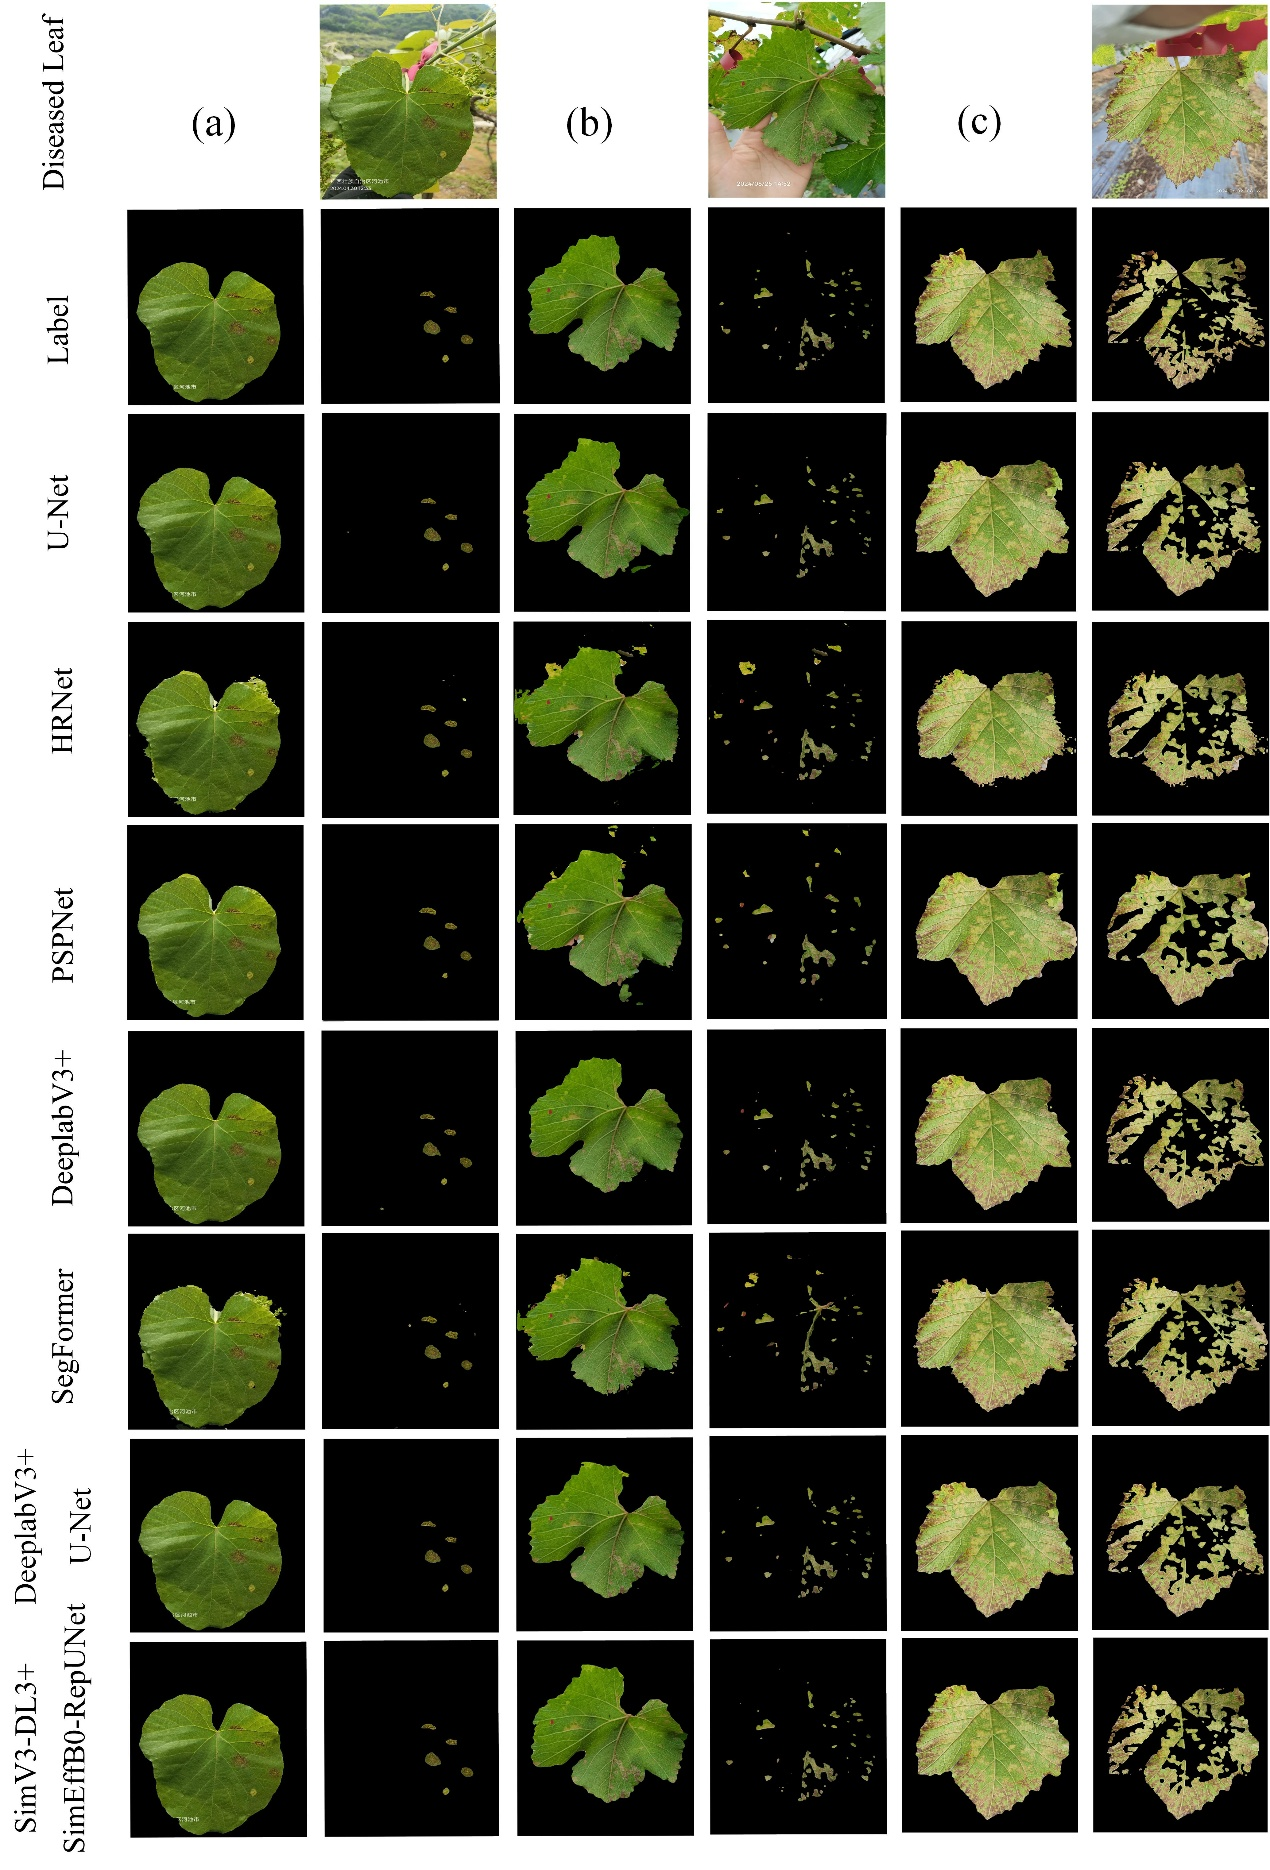
\includegraphics[width=\linewidth,height=0.72\textheight,keepaspectratio]{Supplementary_Materials_media/media/image2.jpeg}
\caption{The actual segmentation results on three images generated by
the five single-stage models and the dual-stage models, including U-Net,
HRNet, PSPNet, DeepLabV3+, SegFormer, DeepLabV3+U-Net, and
SimV3-DL3+SimEffB0-RepUNet.}
\label{fig:s2-segmentation}
\end{figure}

\begin{figure}[htbp]
\centering

\includegraphics[width=0.95\linewidth]{Supplementary_Materials_media/media/image3.png}
\caption{Illustrative comparison of predicted severity with expert
visual estimates, where S1--S15 represent the expert visual estimate,
average for the average value of the total 15 expert estimates, and
predicted for predicted severity with our model.}
\label{fig:s3-expert-comparison}
\end{figure}

\begin{figure}[htbp]
\centering

\includegraphics[width=\linewidth]{Supplementary_Materials_media/media/image4.jpeg}
\caption{The mobile application and its pipeline for leaf disease
severity estimation.}
\label{fig:s4-mobile-application}
\end{figure}

\end{document}
